\documentclass[10pt,a4paper]{article}
\usepackage[utf8]{inputenc}
\usepackage[T1]{fontenc}
\usepackage[spanish]{babel}
\usepackage{amsmath}
\usepackage{amsfonts}
\usepackage{amssymb}
\usepackage{graphicx}
\usepackage{float}
\usepackage{multicol}
\usepackage[dvipsnames]{xcolor}
\usepackage{hyperref}
\definecolor{pinegreen}{rgb}{0.36, 0.54, 0.66}
\hypersetup{
    colorlinks=true,
    linkcolor=pinegreen,      
    urlcolor=red,
    }
\addto{\captionsspanish}{\renewcommand{\abstractname}{Abstract}}
\newcommand{\celda}[1]{
	\begin{minipage}{2cm}
		\vspace{2mm}
		#1
		\vspace{2mm}
	\end{minipage}
}
\definecolor{pinegreen}{rgb}{0.36, 0.54, 0.66}
\usepackage[left=2.00cm, right=2.00cm, top=2.00cm, bottom=2.00cm]{geometry}
%-----------------------
\usepackage{fancyhdr}
\usepackage{lastpage}   
\pagestyle{fancy} 
\fancyhf{}   
\rhead{Gabriel Hernández}                       %Create right header text
\chead{Estimación experimental de $\pi$}  
\lhead{Laboratorio 2}                        %Create left header text
                   %Create center header text

\rfoot{Page \thepage \hspace{1pt} of \pageref{LastPage}}    %Create right footer text
\renewcommand{\headrulewidth}{0.2pt}      %Set header line thickness to 0 pt [default=1pt]
\renewcommand{\footrulewidth}{0pt}      %Set footer line thickness to 0 pt [default =0pt]
%-----------------------
\author{Gabriel Hernandez Bello}
\begin{document}
	
	\begin{figure}[H]
		\raggedright
		
\includegraphics[scale=0.2]{../Altura-Campanil/IMG/logo_udec.png} \hfill 
\includegraphics[scale=0.5]{../Altura-Campanil/IMG/cfm_logo.png}
	\end{figure}

	\vspace{6mm}
	%ESTE CENTER ES EXCLUSIVO PARA EL TITULO DEL PAPER, AUTOR Y UNIVER.
	\begin{center}
		{\Large \textbf{Estimación experimental de \textbf{$\pi$}}}\\
		\vspace{2mm}
		{\large Gabriel Hernández Bello$^{1}$}\\
		\vspace{6.5mm}
		$^1$\textit{Universidad de Concepción, Facultad de Ciencias Físicas y Matemáticas, Ciencias Físicas. }\\
	\end{center}

	\begin{center}
		\textcolor{pinegreen}{\rule{150mm}{0.8mm}}
	\end{center}

      %ESTE ABSTRACT ES PARA EL RESUMEN PROPIAMENTE DICHO Y PARA LAS PALABRAS CLAVES (KEYWORDS) ,NOTA:el comando \par sirve para iniciar el nuevo parrafo con sangría.
	\begin{abstract}
	Se desarrollaron experimentalmente dos métodos para la medición del número $\pi$. El primero se centró en la verificación de la definición de $\pi$, comparando el perímetro de distintos círculos con su diámetro. El segundo método se centró en el cálculo de $\pi$ mediante la comparación de áreas y masas de círculos y cuadrados fabricados con el mismo material.\\
	
	Los valores obtenidos entregaron una estimación de 3.140 $\pm$ 0.006 para el primer método y 3.149 $\pm$ 0.021 para el segundo, con un error relativo de 0.04 $\%$ y un 0.2 $\%$, respectivamente. A pesar de que el segundo método presentó errores que no abarcaron el promedio de los datos, el bajo nivel de error en las estimaciones finales permite concluir que el laboratorio fue realizado exitosamente.

		\textbf{Palabras Claves ---}  $\pi$, estimación, radio, densidad de masa.
	\end{abstract}
	
	\begin{center}
		\textcolor{pinegreen}{\rule{150mm}{0.8mm}}
	\end{center}
	
	\begin{multicols}{2}
		\section{Introducción}
			El número $\pi$ es una de las constantes matemáticas por autonomasia. Su omnipresencia en diferentes ámbitos relacionados con la física, las matemáticas y la ingeniería lo hacen reconocible hasta para aquellos que viven alejados de las ramas científicas.\\
			
			El emblemático número irracional $\pi$ se define como la razón entre el perímetro de una circunsferencia y su diámetro. Toda investigación que incluya alguna variable relacionada con círculos, circunferencias o similares llevará implícito su cálculo, desde las elipses de las trayectorias espaciales hasta la fabricación de ruedas o balones de fútbol. A partir de ahí, su utilidad es casi tan dilatada como su número de decimales \cite{discovery}.\\
			
			En el presente laboratorio, nos concentraremos en estimar experimentalmente el valor del número $\pi$ a través de dos experimentos simples.
		\section{Marco Teórico}
		\subsection*{Definición de $\pi$}
		Sea una circunsferencia con perímetro $P$ y diámetro $D$. Se define el número $\pi$ como la razón entre estas magnitudes \cite{wikipi}, tal que:
		\begin{equation}\label{def de pi}
		\pi = \frac{P}{D}
		\end{equation}
	
		\subsection*{Integrales en la antiguedad}
		Arquímedes de Siracusa (287-212 a.C.) utilizó el método exhaustivo de Euxodo de Cnido. inscribiendo y 	
circunscribiendo polígonos regulares en una circunferencia para calcular áreas y volúmenes. Calculó el volumen y la superficie de una esfera y de un cono y la superficie de una elipse y una parábola y expuso un método para calcular los volúmenes de revolución de segmentos de elipsoides, paraboloides e hiperboloides cortados por un
plano perpendicular al eje principal \cite{integral}. \\

		De esta forma se calculaban las integrales, relacionadas a áreas y volúmenes, en la antiguedad. Esta noción es de suma importancia para el laboratorio, pues en ella esta basada una de los experimentos propuestos para la estimación de $\pi$.
		\subsection*{Relación entre masas y $\pi$}
		Consideremos un material con densidad de masa superficial $\rho$ constante, de forma que $m = \rho A$; donde $m$ representa la masa del material y  $A$ su área. Ahora, recortemos una circunsferencia de radio $a$ y un cuadrado de lado $a$ en el mismo material. Así, el área de la circunsferencia será $A = \pi a^2$ y para el cuadrado tendremos un área de $B = a^2$. Luego, es directo mostrar que:
		\begin{align}
		\rho_a &= \rho_b \\
		\Longrightarrow \frac{m_a}{A} &= \frac{m_b}{B}\\
		\Longrightarrow \frac{m_a}{m_b} &= \frac{A}{B}\\
		\Longrightarrow \frac{m_a}{m_b} &= \pi \label{masa pi}
		\end{align}
		Donde concluímos que la razón entre las áreas del círuclo y el cuadrado resulta en el número $\pi$. \\
		\section{Procedimiento Experimental y Resultados}
		Este laboratorio esta dividido en dos experimentos. Para el primero medimos la circunsferencia de varios círculos y lo camparamos con su respectivo diámetro. Esto corresponde simplemente a la verificación de la definicón del número $\pi$ vista en \ref{def de pi}.\\
		
		\begin{figure}[H]
			\centering
			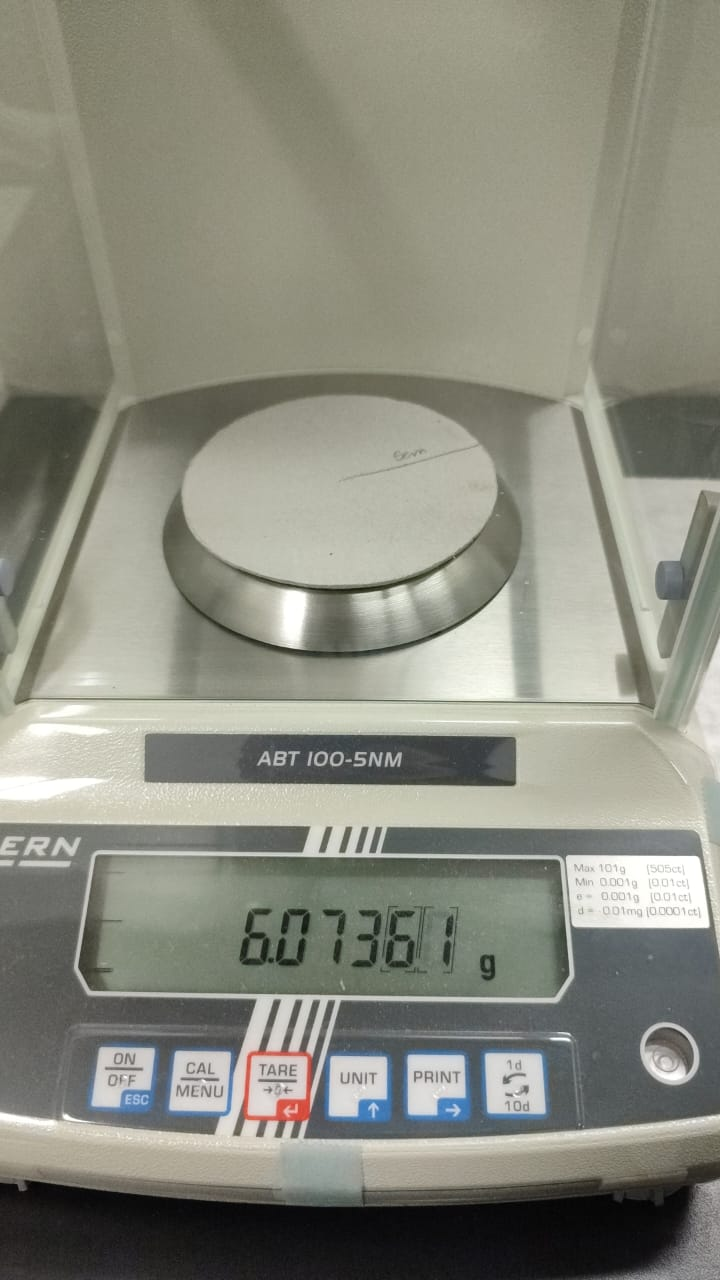
\includegraphics[scale=0.1]{circulo_pi.jpeg}
			\caption{Gráfico de las mediciones para el segundo método.}
			\label{Mediciones foto}
			\rule{80mm}{0.1mm}
		\end{figure}
		
		
		Para el segundo experimento, nos basamos en la forma antigua del cálculo de integrales. Dicha forma consiste en realcionar áreas y volumenes a través de la medición y comparación de la masa de estos objetos correspondientes. En nuestro caso, decidimos comparar círuclos y cuadrados, del mismo material, con un radio y largo correspondientes, de forma que sea válido aplicar los resultados destacados anteriormente \ref{masa pi}. Cabe destacar que para la recolección de datos sobre la masa de los distintos objetos usamos una balanza analítica ABT 100-5NM que presentaba una sensibilidad de $10^{-5}$ [g], ver figura \ref{Mediciones foto}.\\
		
		En los cuadros \ref{tab:primer exp} y \ref{tab:segundo exp} se recogen los datos obtenidos para el primer y segundo experimento, respectivamente. Cabe destacar que el error asociado a la medida del número $\pi$  en ambos casos fue calculado de manera analítica con la siguiente fórmula \cite{error}:
		\begin{equation}\label{errores}
		\sigma^2 = \sigma^2_x \left( \frac{\partial f}{\partial x} \right)^2 + \sigma^2_y \left( \frac{\partial f}{\partial y} \right)^2 + \sigma^2_z \left( \frac{\partial f}{\partial z} \right)^2+...
		\end{equation}
		\end{multicols}
		
			
		\begin{table}[H]
			\centering
			\begin{tabular}{|c|c|c|c|}
				\hline
				Radio (cm) & Perímetro(cm) &  $\pi$ \\ \hline
				4.00 $\pm$ 0.05  & 25.20 $\pm$ 0.05  & 3.15 $\pm$ 0.03 \\
				4.50 $\pm$ 0.05  & 28.20  $\pm$ 0.05 & 3.13 $\pm$ 0.03\\
				5.00 $\pm$ 0.05  & 31.40 $\pm$ 0.05 & 3.14 $\pm$ 0.03 \\ 
				8.00 $\pm$ 0.05  & 50.20 $\pm$ 0.05 & 3.13 $\pm$ 0.02\\ \hline
			\end{tabular}
			\caption{Datos del radio, perímetro y valor estimado de $\pi$ para el primer experimento.}
			\label{tab:primer exp}
			\rule{100mm}{0.1mm}
		\end{table}
		
		\begin{table}[H]
			\centering
			\begin{tabular}{|c|c|c|c|}
				\hline
				Radio (cm) & Masa círculo (g) & Masa caudrado (g) & $\pi$ \\ \hline
				4.00 $\pm$ 0.05  & 1.02603 $\pm$ 0.00001 & 0.33134 $\pm$ 0.00001 & 3.09661 $\pm$ 0.00009 \\
				4.50 $\pm$ 0.05  & 1.50946  $\pm$ 0.00001 & 0.48270 $\pm$ 0.00001 & 3.12711 $\pm$ 0.00006\\
				5.00 $\pm$ 0.05  & 6.07361 $\pm$ 0.00001 & 1.88232 $\pm$ 0.00001 & 3.22666 $\pm$ 0.00001 \\ 
				8.00 $\pm$ 0.05  & 14.97495 $\pm$ 0.00001 & 4.75779 $\pm$ 0.00001 & 3.14745 $\pm$ 0.00006\\ \hline
			\end{tabular}
			\caption{Datos del radio, masas del círculo y el cuadrado, y el valor estimado de $\pi$ para el segudo experimento.}
			\label{tab:segundo exp}
			\rule{100mm}{0.1mm}
		\end{table}
		
	\begin{multicols}{2}
	\section{Análisis}
	En las figuras 1 y 2 se grafican los valores obtenidos para el primer y segundo experimento, respectivamente. Del análisis de las gráficas resulta evidente que el primer método de medición es mucho mas preciso, acercándose considerablemente al valor real del número $\pi$ , en comparación al segundo método.\\
	
	De la gráfica 2, notamos que las barras de error no abarcan el valor promedio de los datos. Adjudicamos este comportamiento al instrumento de medición utilizado, pues entregó resultados  con un orden de magnitud de $10^{-5}$ minimizando el error de la medición, pero dispersando el valor de los datos, lo que se refleja en una desviación estándar de 0.02 notablemente superior a la desviación del primer método con un 0.006. Más aún, destacamos que la elección de un material no tan pesado (cartón), como también la forma poco minuciosa de recortar los círculos influyeron en la presición del experimento.\\
	
	Pese a lo anteriror, en rasgos generales, los valores estimados de $\pi$ estuvieron relativamente próximos a su valor teórico. En efecto, considerando el valor promedio y la desviación estándar para cada método, se obtuvo:
	\begin{align}
	\pi_1 & = 3.140 \pm 0.006 \\
	\pi_2 & = 3.149 \pm 0.021
	\end{align}
	
	\begin{figure}[H]
			\centering
			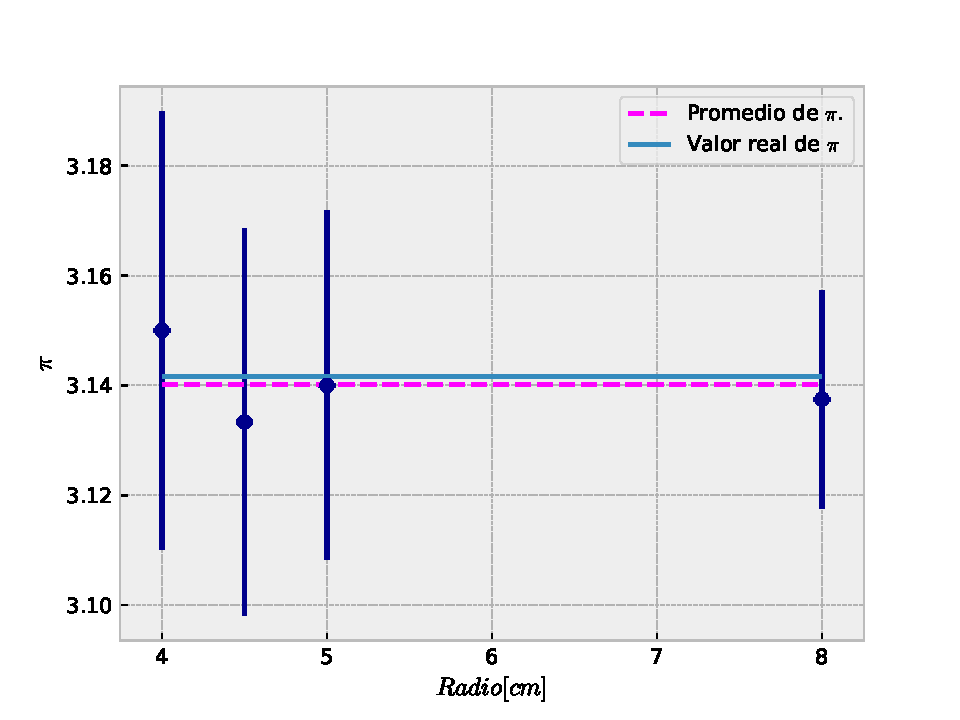
\includegraphics[scale=0.5]{pi_metodo1.pdf}
			\caption{Gráfica de el valor estimado de $\pi$ respecto al radio de los círculos para el primer experimento.}
			\label{imagen primer exp}
			\rule{80mm}{0.1mm}
		\end{figure}
		
		\begin{figure}[H]
			\centering
			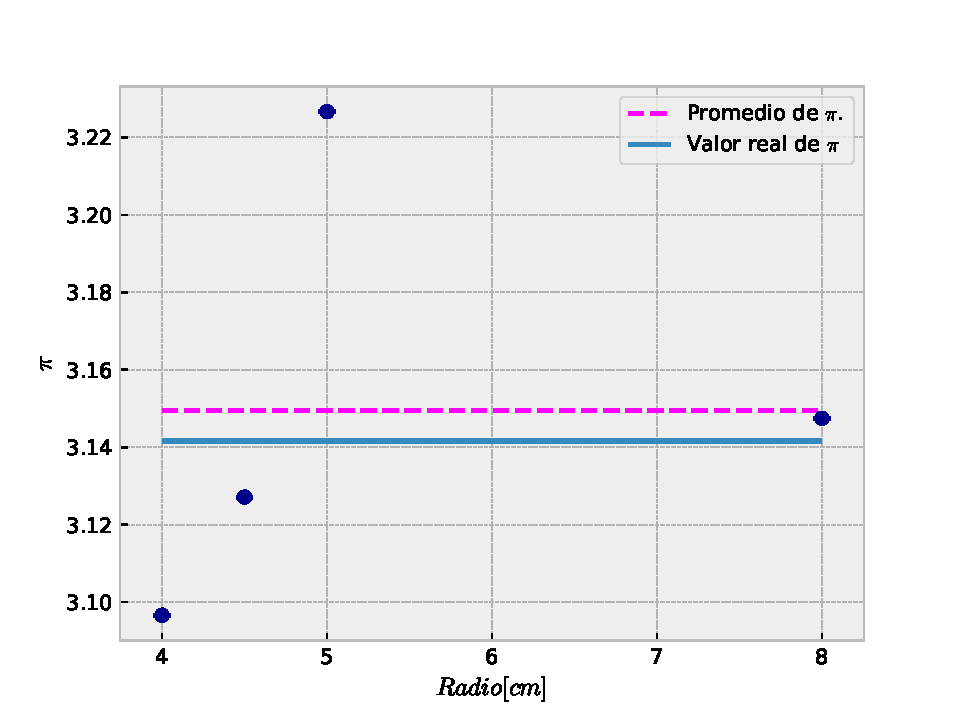
\includegraphics[scale=0.5]{pi_metodo2.pdf}
			\caption{Gráfica de el valor estimado de $\pi$ respecto al radio de los círculos y cuadrados para el segundo experimento.}
			\label{imagen segundo exp}
			\rule{80mm}{0.1mm}
		\end{figure}
	
\section{Conlusión}
En el presente laboratorio mostramos dos métodos para la estimación experimental del número $\pi$. Durante el análisis de los datos obtenidos, notamos que el primer experimento entregó valores congruentes y cercanos al valor teórico de $\pi$. Por otra parte, el segundo experimento, si bien entregó valores próximos al valor real de $\pi$, los errores asociados a la medición no abarcaban el valor promedio de los datos. Este comportamiento puede atribuirse a factores como la elección del instrumento de medición, el material utilizado y la presición en el  corte de los círculos, los cuales terminaron afectando a la presición global de los resultados.\\

Para mejorar la congruencia en los datos del segundo método, recomendamos utilizar un instrumento de medición más adecuado, pues para este experimento en partiular no era necesaria una presición excesiva. Además el  uso de un material más pesado podría ayudar a reducir el error asociado al corte irregular del círculo, minimizando así su influencia en resultado general.\\

A pesar de estas limitaciones, se obtuvieron resultados cercanos al valor teórico de $\pi$ con una estimación de 3.140 $\pm$ 0.006 para el primer método y 3.149 $\pm$ 0.021 para el segundo. Lo anterior se traduce en un error relativo de 0.04 $\%$ para el primer método y un 0.2 $\%$ para el segundo. De esta forma, dado el baja nivel de de error presente en los resultados, concluímos que el laboratorio fue llevado a cabo con éxito.





	\bibliographystyle{unsrt}
	\bibliography{referencias}
	
	\end{multicols}
\end{document}